\begin{frame}
  \frametitle<1| handout:1>{A simple picture of X-ray absorption} 
  \frametitle<2| handout:2>{X-ray absorption in condensed matter}

  \begin{overlayarea}{\linewidth}{6ex}
    \only<1| handout:1>{An incident x-ray of energy $E$ is absorbed,
      destroying a core electron of binding energy $E_0$ and emitting
      a photo-electron with kinetic energy $(E-E_0)$. The core state
      is eventually filled, ejecting a fluorescent x-ray or an Auger
      electron.  }%
    \only<2| handout:2>{The ejected photo-electron can scatter from
      neighboring atoms. $R$ has some relationship to $\lambda$ and
      there is a phase shift associated with the scattering event.
      Thus the outgoing and scattered waves interfere.  }%
  \end{overlayarea}

  \vskip 20pt

  \begin{columns}[T]
    \begin{column}{0.5\linewidth}
      \only<1| handout:1>{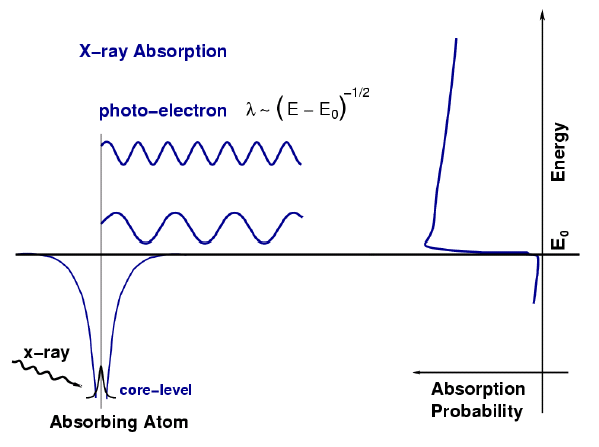
\includegraphics[width=\linewidth]{bare_atom.png}}
      \only<2| handout:2>{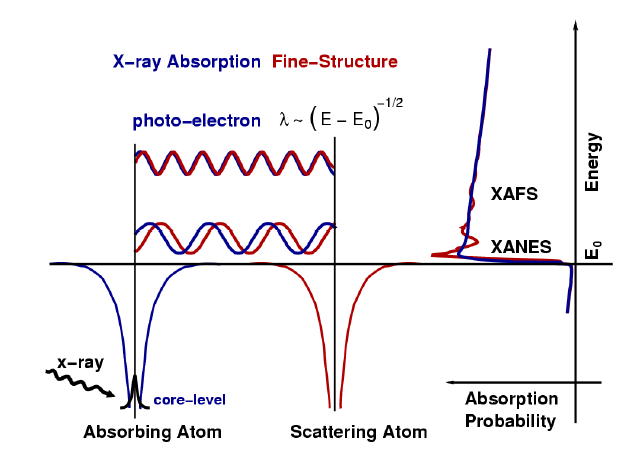
\includegraphics[width=\linewidth]{with_scattering.png}}
    \end{column}
    \begin{column}{0.5\linewidth}
      \begin{center}
        \only<1| handout:1>{
          An empty final state is required.\\
          {\alert{No available state, \\
              no absorption!}}\\
          When the incident x-ray energy is larger than the binding
          energy, there is a sharp increase in absorption.
        }
        \only<2| handout:2>{
          The scattering of the photo-electron wave function interferes
          with itself.\\[4ex]
          $\mu(E)$ depends on the density of states with energy
          $(E-E_0)$ at the absorbing atom.
        }
      \end{center}
    \end{column}
  \end{columns}

  \vskip 20pt

  \begin{overlayarea}{\linewidth}{3ex}
    \only<1| handout:1>{For an isolated atom, $\mu(E)$ has a sharp step at the
      core-level binding energy and is a smooth function of energy
      above the edge.}%
    \only<2| handout:2>{This interference \alert{at the absorbing atom} will vary
      with energy, causing the oscillations in $\mu(E)$.
    }%
  \end{overlayarea}
  \begin{bottomnote}[0.7][20] 
    Image from Matt Newville
  \end{bottomnote}
\end{frame}
